\documentclass[10pt]{book}
\usepackage{amsmath}
\usepackage{mathspec}
\usepackage{sectsty, titlesec}
\usepackage{wrapfig, booktabs}
\usepackage{nomencl}
\makenomenclature
\renewcommand{\nomname}{List of symbols and\\abbreviations}
\usepackage[numbers]{natbib}
\usepackage{graphicx,caption,subcaption}
\setmainfont[Mapping=tex-text]{Crimson}
\setsansfont[Scale=0.88]{Alte DIN 1451 Mittelschrift}
%\allsectionsfont{\sffamily}
%\setmainfon
%\usepackage{fouriernc}
%\usepackage[T1]{fontenc}
\setmathsfont(Digits,Latin){Crimson}
\setmathrm[BoldFont={Crimson Bold}]{Crimson}
\setmathsfont(Greek)[Scale=1.15]{Crimson}

% Character shortcuts
\newcommand*{\Hhat}{\hat{\vphantom{\scalebox{1.2}{H}} H}}
\newcommand*{\Phat}{\hat{\vphantom{\scalebox{1.2}{P}} P}}


\usepackage{fancyhdr}
\setlength{\headheight}{15pt}
\setlength{\marginparwidth}{1.2in}
%\titleformat{\section}{\huge\sansnormalfont}{\protect\makebox[0pt][r]{\thesection\quad}}{0em}{}
\titleformat{\chapter}{\fontsize{32pt}{36pt}\selectfont\bfseries}{}{0em}{}
\titleformat{\section}{\fontsize{18pt}{22pt}\selectfont\bfseries}{\protect\makebox[0pt][r]{\thesection\quad}}{0em}{}
\titleformat{\subsection}{\fontsize{12pt}{16pt}\selectfont}{\protect\makebox[0pt][r]{\thesubsection\fontsize{18pt}{22pt}\selectfont\quad}}{0em}{}
%\titleformat{\paragraph}{\fontsize{12pt}{16pt}\selectfont}{}{}{}
\pagestyle{fancy}
\renewcommand{\chaptermark}[1]{ \markboth{#1}{} }
\renewcommand{\sectionmark}[1]{ \markright{#1}{} }

\fancyhf{}
\fancyhead[LE,RO]{\sffamily\thepage}
\fancyhead[RE]{\sffamily{ \nouppercase{\leftmark}} }
\fancyhead[LO]{\sffamily{ \nouppercase{\rightmark}} }

\fancypagestyle{plain}{ %
  \fancyhf{} % remove everything
  \renewcommand{\headrulewidth}{0pt} % remove lines as well
  \renewcommand{\footrulewidth}{0pt}
}

\parskip 0pt
%\usepackage{xunicode}
\begin{document}
\title{Experimental verification\\ of the IPI sizing technique}
\author{Sebastian Kosch}
\date{July 2014}
\maketitle

\printnomenclature[5em]

\chapter{Introduction}
\section{Why spray sizing is important}
\section{What our contributions in this paper are}
- Our contributions:
    - Pupillary magnification has to be taken into account
    - Circle detection algorithm is crap
\section{What other work has been done in this area}

\chapter{Experimental setup}
- Our setup:
\section{Dantec system}
    - Dantec system
\section{PDPA system}
    - TSI system
\section{Droplet generator}
\label{sec:droplet-generator}
    - Droplet generator
\section{Verification of droplet sizes}
    - This is where I show pictures and tables, showing that the formula
    actually works.

    \chapter{Interferometric Particle\\ Imaging (IPI)}
\section{Operating principle}
The number of fringes $N_\text{fr}$ appearing in the image has a simple linear relationship to
the droplet diametre $D_d$:
\nomenclature{$N_\text{fr}$}{Number of fringes}
\nomenclature{$\kappa$}{Scalar value relating the fringe count $N_\text{fr}$ to
the physical diameter of the particle $D_d$}
\nomenclature{$D_d$}{Physical diameter of the particle (here: droplet)}
\begin{equation}
    N_\text{fr} = \kappa D_d,
\end{equation}
where $\kappa$ is a constant derived from the optical configuration:
\begin{equation}
    \kappa = \frac{\arcsin\left(\frac{D_a}{2z}\right)}{\lambda}
    \left(\cos\frac{\phi}{2} - \frac{m \sin\frac{\phi}{2}}{\sqrt{m^2 + 1 -
    2m\cos \frac{\phi}{2}}}\right).
    \label{kappa}
\end{equation}

In the above expression $D_a$ is the aperture diametre, $z$ is the distance of
the lens to the laser sheet, $\phi$ is the off-axis angle (90 degrees in most
setups, including ours), and $m$ is the relative refractive index of the
droplets (1.333 for water in air).

As a consequence of geometrical optics, the distance $s_x$ (in pixels) between two
adjacent fringes has a linear relationship with the defocussing distance $\Delta
z$, where $M$ is the magnification, $d_{p,x}$ is the physical size of a
camera sensor pixel, and $\Delta \theta$ is the angle subtended by two adjacent
fringes entering the lens \cite{Pan06}:
\nomenclature{$\Delta \theta$}{Angular spacing between two adjacent fringes}
\nomenclature{$\Delta z$}{Distance along the $z$-axis between the focal plane of
the lens and the light sheet}
\nomenclature{$M$}{Magnification}
\nomenclature{$s_x$}{Distance, in pixels, between two adjacent fringes}
\nomenclature{$d_{p,x}; d_{p,y}$}{Physical dimensions of a pixel on the camera's
CCD sensor}
\begin{equation}
  s_x = \frac{\Delta \theta \Delta z}{M d_{p,x}} 
  \label{fringedistance-pixels}
\end{equation}
Of course, equation \eqref{fringedistance-pixels} is only meaningful where $\Delta z \gg
0$. If the image is (approximately) focussed, fringes will give way to a sharp
image of either both glare points or a single bright spot -- depending on
diffraction effects and the camera's resolution.

(Fill in more details here.)

\section{Setup}
\label{sec:ipi-setup}
(How it's set up, what cameras, what lenses, what laser, timer box, software,
etc.)

\section{Common problems and sources of error}
\subsection{Too much overlap}
\label{sec:ipi-overlap}
This is a section where I refer to the paper that calculates overlap
probabilities. I explain that many droplets are mis-identified (either high-freq
is seen as low-freq, or noise is seen as high-freq) and where I point out that
while Hanning windows and min-distance/max-overlap filters help a little bit,
they also skew the representativeness of the sample because only small,
dispersed satellites are outside of the main flow.

I explain that there isn't really an easy method of fixing this, and that any
time spent attempting to deal with the problem is better spent building a slit
aperture system, as described in the next chapter.

\subsection{Droplet detection and camera mapping}
The most challenging stage of the measurement process is the detection of the
defocussed droplet images. Since the defocussed images assume the shape of the
aperture, which is wide open in most applications,\footnote{see Chapter
\ref{chapter:slitaperture} for a discussion of the benefits of non-circular
apertures.} they are typically circular. Moreover, they are all more or less of
the same size as a consequence of equation \eqref{}.

\begin{figure}
\centering
%\includegraphics[]{droplet-overlap.jpg}
\caption{Overlapping defocussed droplet images}
\label{fig:droplet-overlap}
\end{figure}

It thus stands to reason that a simple circle detection technique would suffice
to detect the droplet images in the photos. A polar adaptation of the Hough
accumulator technique (such as the OpenCV implementation
\texttt{cv2.HoughCircles()}) or a correlation-based pattern matching method
(e.g. \texttt{cv2.matchTemplate()}) are both obvious choices for this task.  The
problem of \emph{droplet overlap}, however, can thwart such efforts (Figure
\ref{fig:droplet-overlap}). This happens particularly when large droplets are to
be measured, because their many fringes require larger defocussed images to
resolve clearly. Indeed, in regions of high droplet density, it can be impossible
to reliably detect the circular fringe images using the methods mentioned above.

Nevertheless, once droplet image positions are established with confidence, overlap can be
dealt with to a degree: known overlapping regions can either be excluded
entirely or serve to help find maximum-likelihood frequency peaks for their
respective tributary droplet images.

Since the detection of droplet images is so essential, the Dantec DynamicStudio
software extracts the droplets' positions from the focussed photo, and then maps
those positions onto the defocussed photo based on a set of camera calibration
photos. This method is sound in principle, but often yields unsatisfactory
mappings in practice, likely whenever the calibration target plate (Figure
\ref{fig:dottarget}) is not precisely aligned with the laser sheet. In section
\ref{sec:calibration-improvement}, we describe a more accurate and robust method
of finding the mapping based directly on the pair of droplet photos. 

Since the mapping error is often a perspectivity, the simple manual
$x/y$-shift that can be applied in the DynamicStudio software after calibration
is not a sufficient adjustment.

Dantec supplies a \emph{standard dot target}, a white $10 \times 10\,
\mathrm{cm}^2$ plate engraved with a pattern of black dots (Figure
\ref{fig:dottarget}). The plate is to be mounted such that its surface coincides
perfectly with the laser sheet. Both cameras are then focussed on the dot
pattern, and a photo is taken with both. This allows the DynamicStudio software
to calculate the transformation matrix between target plate and
image for each camera:
\begin{equation}
\left[\begin{array}{c} x'\\ y'\\ z'\\ r' \end{array} \right]
=
\left[ \begin{array}{cccc}
S_x & A_{yx} & A_{zx} & T_x \\
A_{xy} & S_y & A_{zy} & T_y \\
A_{xz} & A_{xy} & S_z & T_z \\
P_x & P_y & P_z & S_0
\end{array} \right]
\left[ \begin{array}{c} x\\ y \\ z \\ 1 \end{array} \right].
\end{equation}

In practice, $P_{x,y,z} = 0$ and $S_z = S_0 = 1$, such that the mapping is
affine (although we will later show that this need not be the case). The
$z$-components (third row/column) are ignored, such that a $3 \times 3$ matrix
suffices for the purposes of this discussion:
\begin{equation}
\left[\begin{array}{c} x'\\ y'\\ r' \end{array} \right]
=
\left[ \begin{array}{ccc}
S_x & A_{yx} &  T_x \\
A_{xy} & S_y &  T_y \\
P_x & P_y & S_0
\end{array} \right]
\left[ \begin{array}{c} x\\ y \\ 1 \end{array} \right].
\end{equation}

The DynamicStudio software thus finds the camera matrices
$\mathbf{P}_\text{foc}$ and $\mathbf{P}_\text{def}$ mapping the
object (the target plate) onto the two camera images:\footnote{Henceforth, the
    subscripts ``foc'' and ``def'' shall designate the focussed and defocussed
    cameras, respectively -- even though both are focussed when the initial
calibration photo is taken.}
\begin{align}
    \mathbf{x}_\text{foc}' &= \mathbf{P}_\text{foc} \, \mathbf{x} \\
    \mathbf{x}_\text{def}' &= \mathbf{P}_\text{def} \, \mathbf{x}.
\end{align}

It follows that the quotient of the two matrices, also known as the homography
\begin{equation}
    \mathbf{H} = \mathbf{P}_\text{def} \, \mathbf{P}_\text{foc}
\end{equation}
can be used to map the focussed image onto the defocussed image:
\begin{equation}
    \mathbf{H}\, \mathbf{x}_\text{foc}' = \mathbf{x}_\text{def}'.
    \label{homography-definition}
\end{equation}

In practice, it is not always possible to ensure that the dot target plate is
aligned with the laser light sheet to absolute perfection. This introduces a
perspective error in the homography matrix $\mathbf{H}$. Figure
\ref{fig:plate-calibration} shows that even though the calibration images
are mapped perfectly, there is a perspective error in Figure
\ref{fig:drop-calibration-off}.

\begin{figure}
        \centering
        \begin{subfigure}[b]{0.45\textheight}
                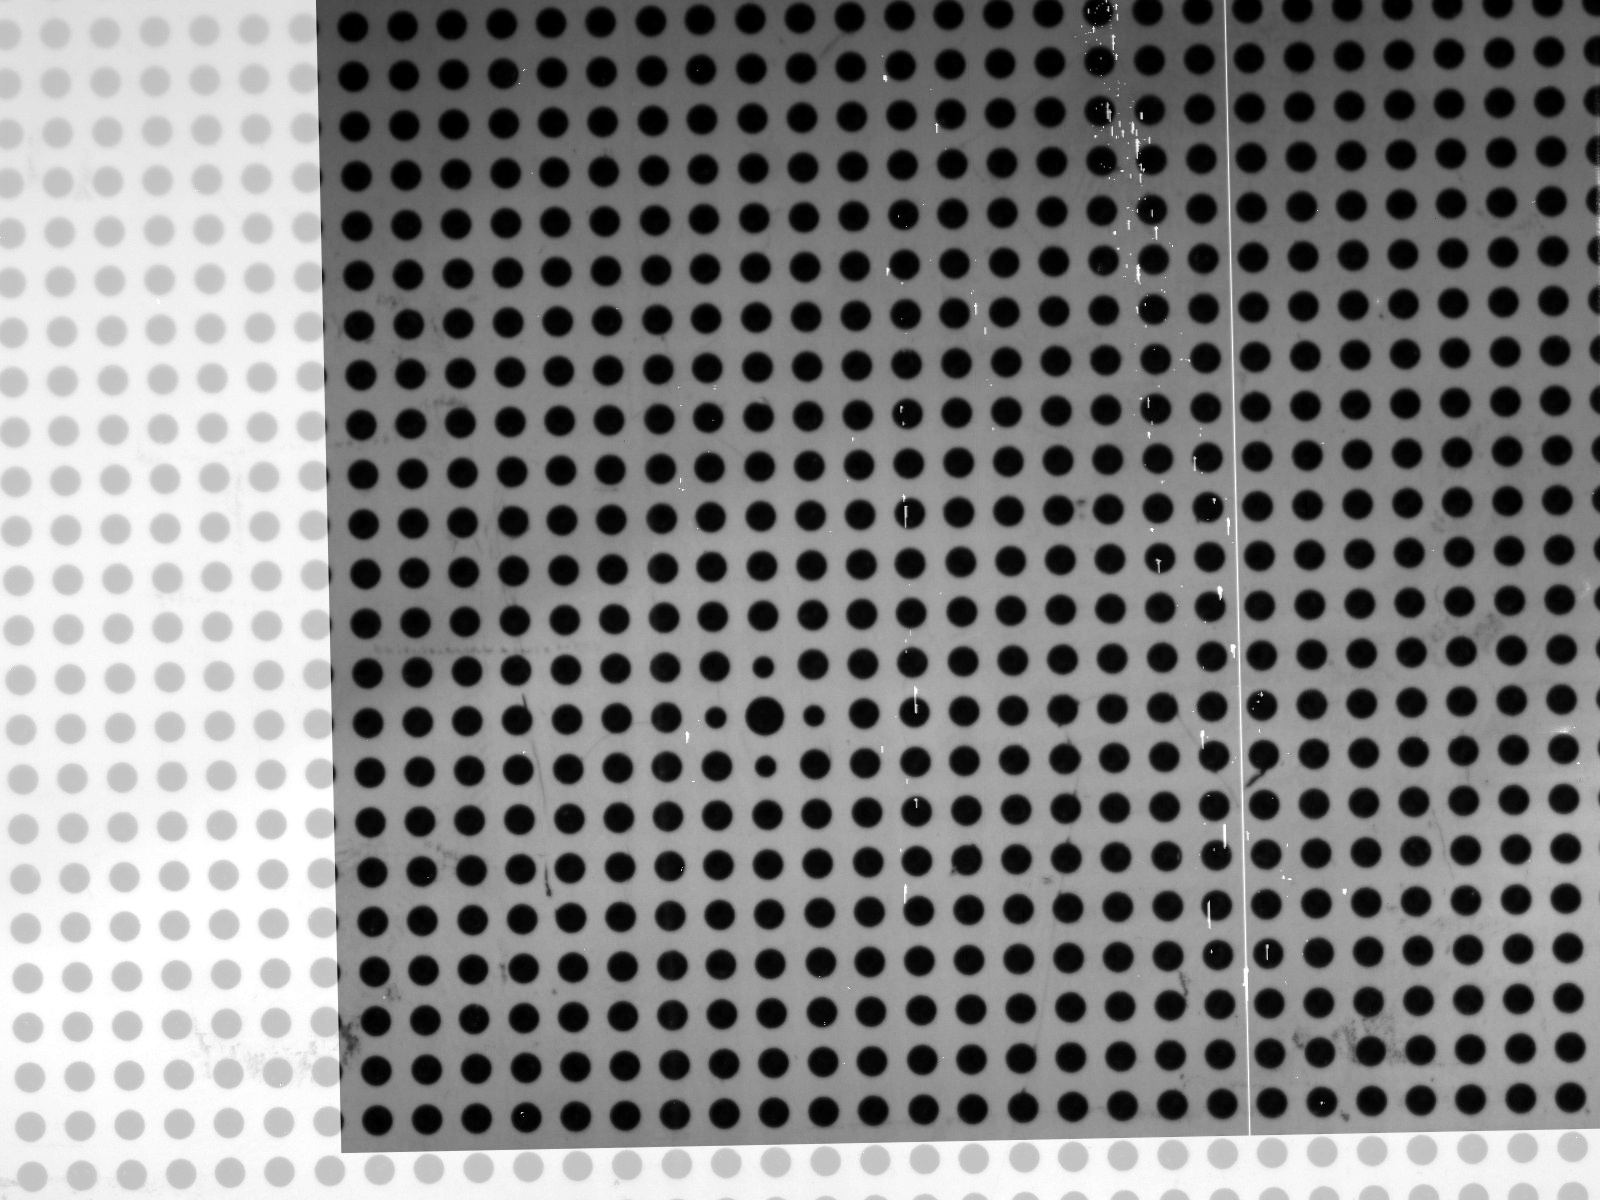
\includegraphics[height=0.4\textheight]{img/plate-calibration.jpg}
                \caption{Focussed camera image, after applying homography, is
                    superimposed onto defocussed camera image of dot target
                plate.}
                \label{fig:plate-calibration}
        \end{subfigure}
        \vskip 2.5em
        \begin{subfigure}[b]{0.45\textheight}
            \centering
                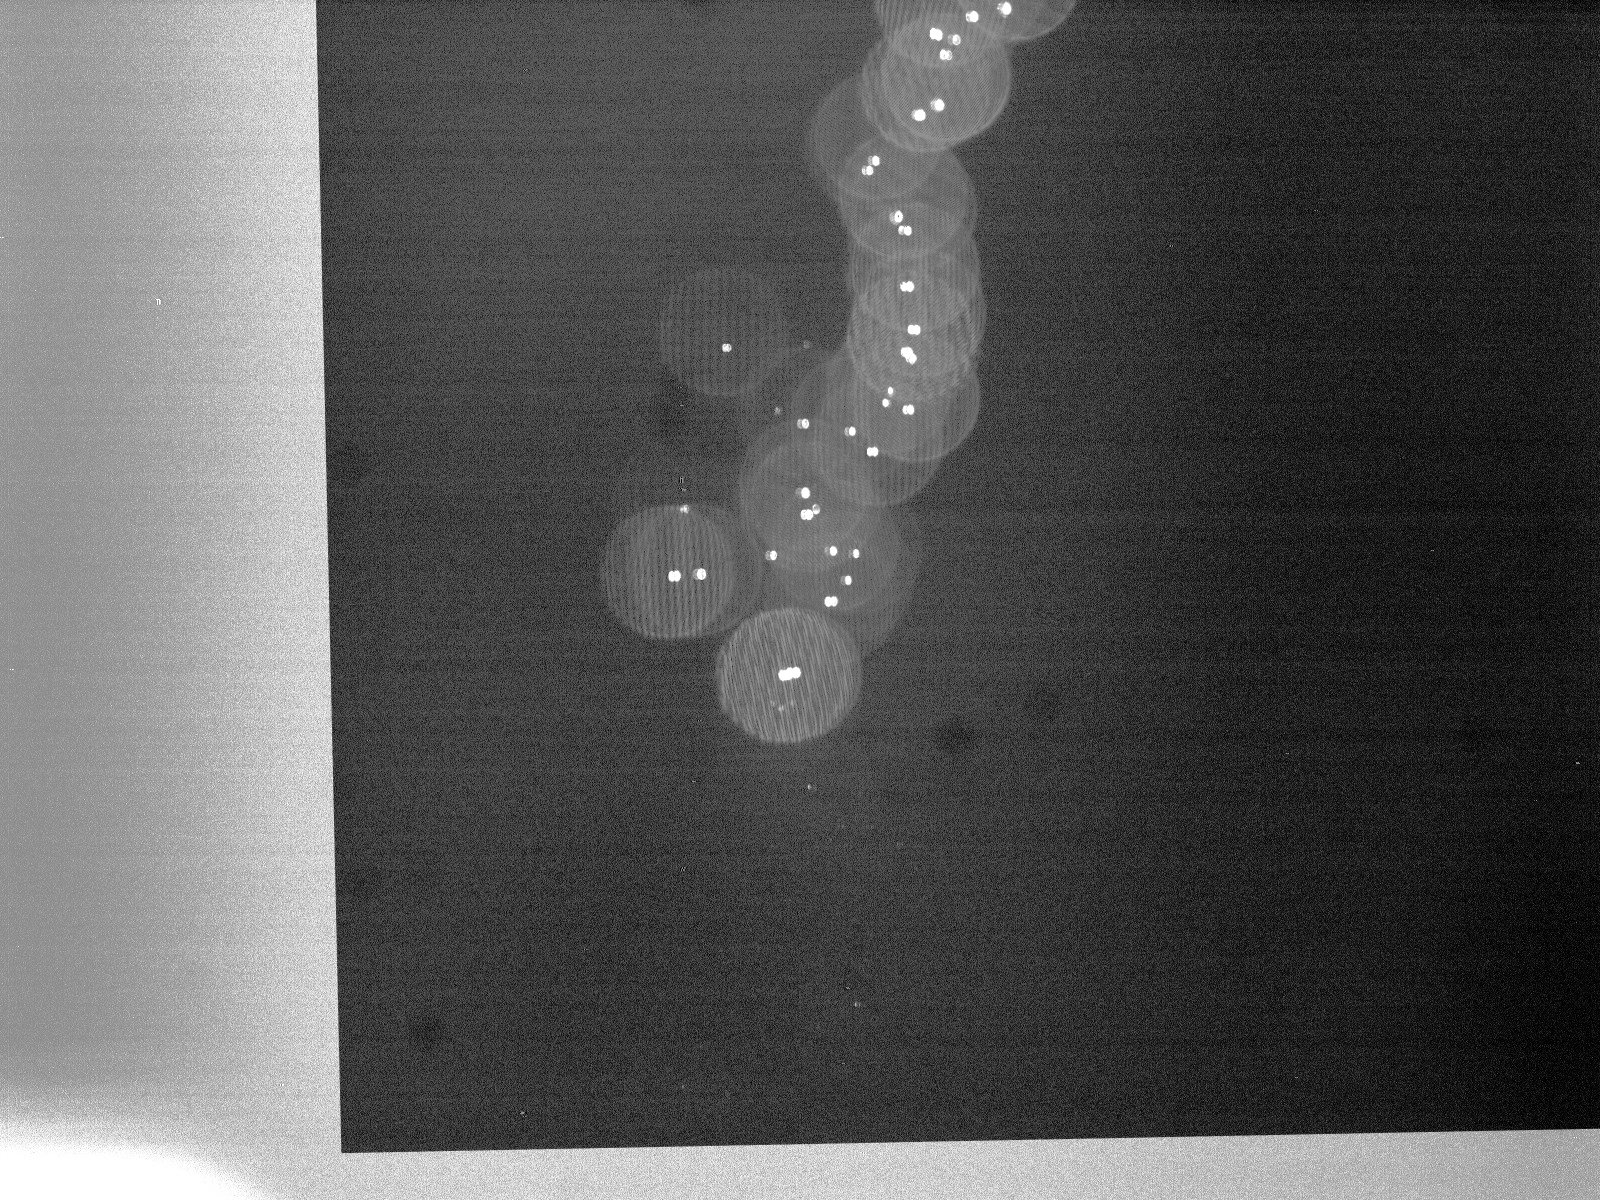
\includegraphics[height=0.4\textheight]{img/drop-calibration-off.jpg}
                \caption{Focussed camera image, after applying homography
                    derived from the calibration images, is superimposed onto
                defocussed camera image of droplets.}
                \label{fig:drop-calibration-off}
        \end{subfigure}
        \caption{Illustration of the perspective error from misaligned
        calibration target plate}
        \label{fig:calibration-error}
\end{figure}

To correct for this error, we can use image registration techniques to derive
the homography mapping \emph{directly} from the focussed and defocussed droplet
images, doing away with the need for calibration pictures altogether. Once we
find the corrected homography $\mathbf{\Hhat}$, we use it to find
\begin{equation}
    \mathbf{\Phat}_\text{def} = \mathbf{\Hhat} \, \mathbf{P}_\text{foc},
    \label{corrected-homography-use}
\end{equation}
which can be manually entered into the DynamicStudio software to replace
$\mathbf{P}_\text{def}$.

\subsubsection{Finding the corrected homography}
Image registration is the process of finding the best possible mapping of one
image onto another -- in other words, it is a term for homography-finding
techniques. The basic process comprises three steps:
\begin{enumerate}
    \item \textbf{Feature detection:} Finding ``features'', i.e. unique points or regions in the images --
        such as corners, arcs, or contrasting regions which stay
        relatively stable even when the image is thresholded.
    \item \textbf{Feature description:} Converting the detected features into
        numerical vectors.
    \item \textbf{Feature matching:} Finding good correspondences between
        features in the two images -- this often requires inlier/outlier
        decision-making, e.g. RANSAC.
\end{enumerate}

Naturally, image registration is impossible to achieve between our focussed and
defocussed images. We therefore first apply the following steps to our focussed
image:

\begin{enumerate}
    \item Mask the image, excluding all areas that are known not to contain
        droplets.
    \item Subtract the pixel-wise minimum or mean taken over all images taken by
        the camera. This step will remove hot pixels on the camera's CCD sensor
        and other static noise.
    \item Erode the image, using a $3 \times 3$ or $5 \times 5$ kernel. This
        will close any remaining bright pixels which are likely noise.
    \item Locate the intensity peaks in the remaining image.
    \item Fill a new image with black, then draw white circles of diameter $D_d$
        onto it, centered at the respective positions of the intensity peaks
        detected in the focussed image.
\end{enumerate}

The result of these operations is shown in Figure \ref{fig:dilating-droplet-dots}.
\begin{figure}
        \centering
        \begin{subfigure}[b]{0.45\textheight}
                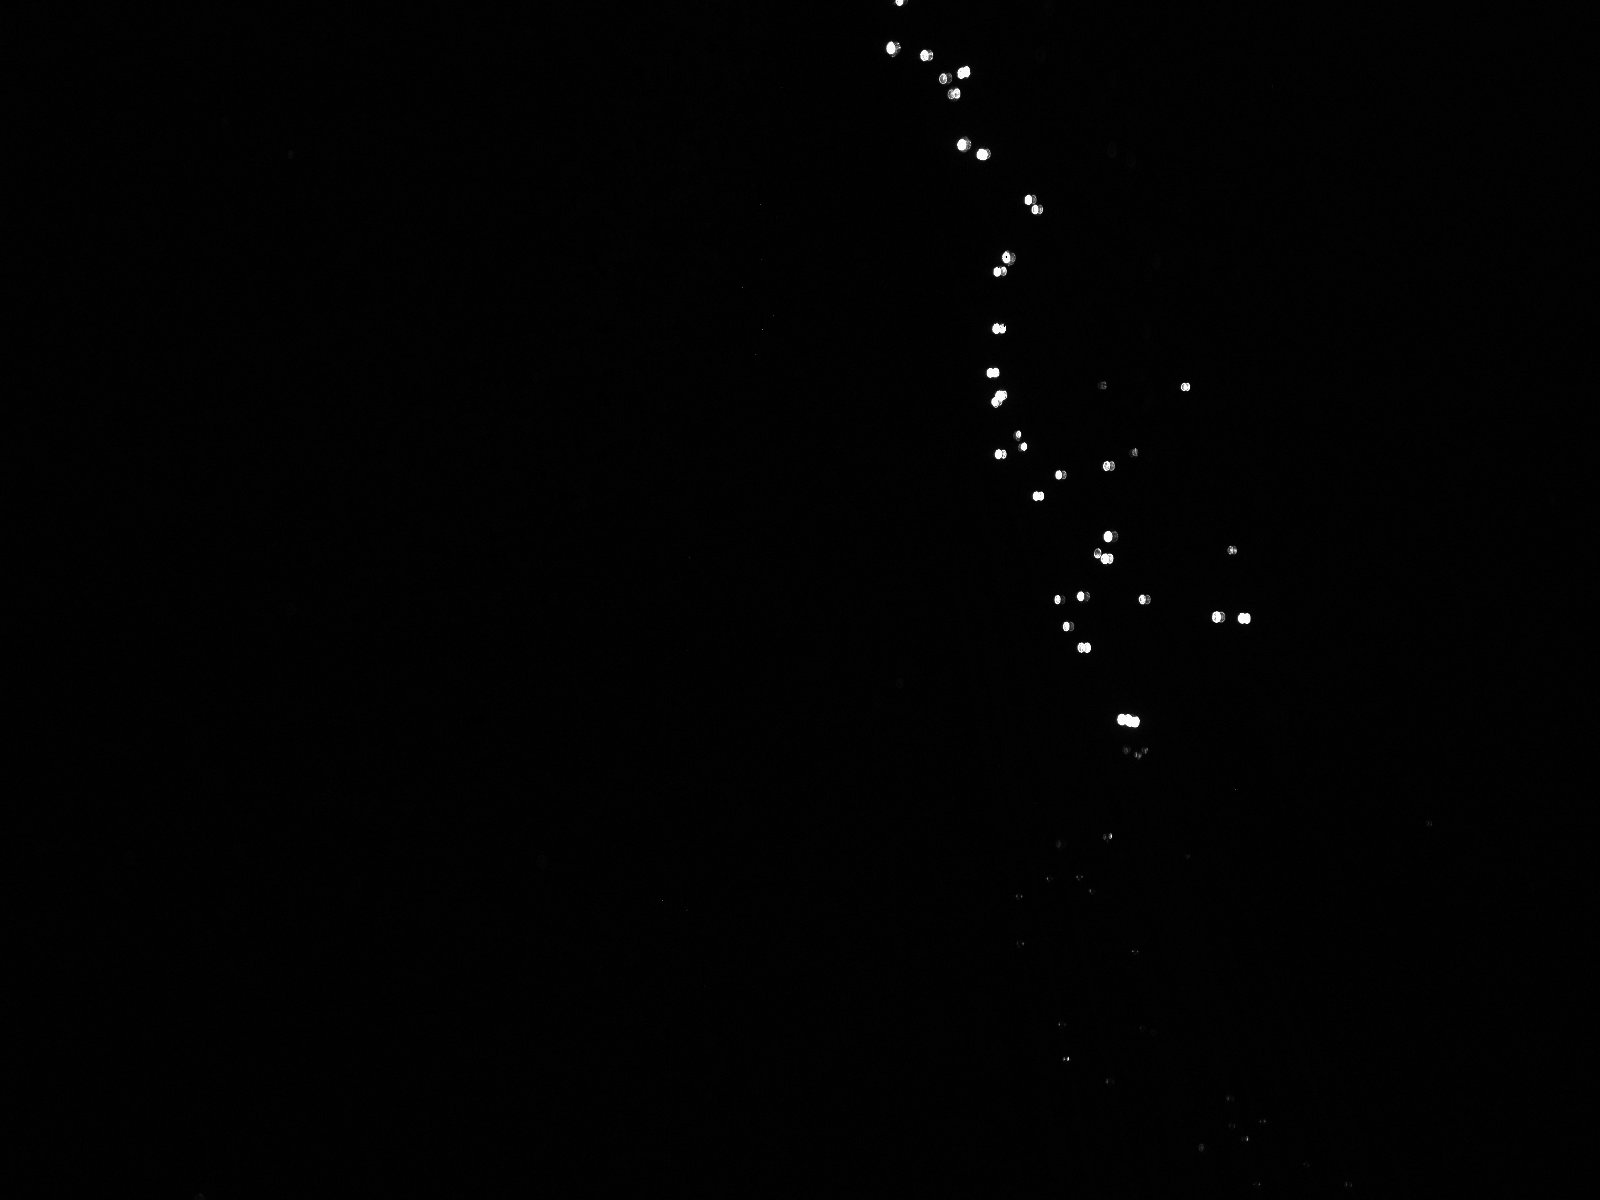
\includegraphics[height=0.4\textheight]{img/focussed.jpg}
                \caption{Focussed camera image.}
                \label{fig:focussed}
        \end{subfigure}
        \vskip 2.5em
        \begin{subfigure}[b]{0.45\textheight}
            \centering
                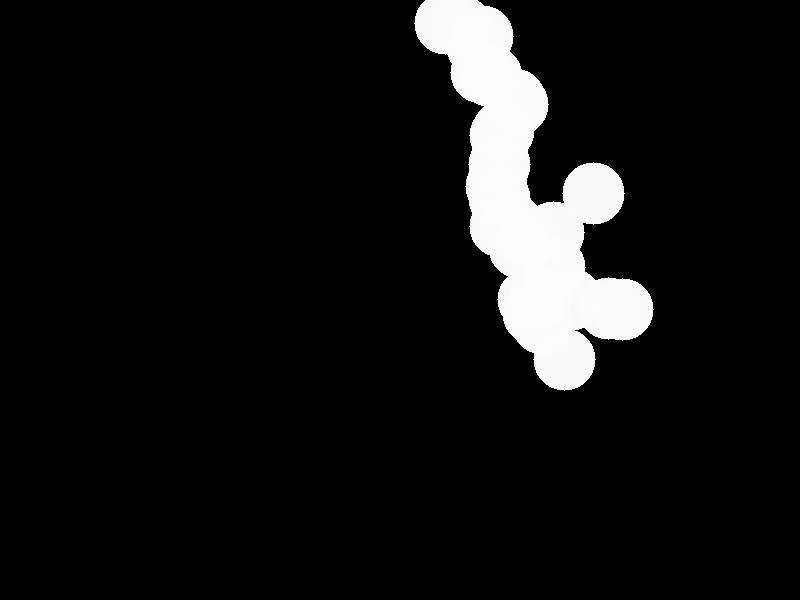
\includegraphics[height=0.4\textheight]{img/focussed-dilated.jpg}
                \caption{Simulated defocussed camera image based on focussed
                camera image, used for registration.}
                \label{fig:focussed-dilated}
        \end{subfigure}
        \caption{Using the focussed image to simulate the defocussed image for
        registration}
        \label{fig:dilating-droplet-dots}
\end{figure}

Image registration algorithms are often not very robust. This is especially true
when the two pictures are not photos taken from slightly different angles.
Moreover, image processing algorithms have runtime complexities that grow at
least with the area of the image. We therefore prepare our focussed image by
shrinking it to half the size (transformation $\mathbf{S}_{0.5}$) and mirroring
it horizontally (transformation $\mathbf{M}_h$).

Our image registration algorithm makes use of the affine invariance of the
\textsc{asift}
algorithm \cite{}, but instead of the patented \textsc{sift} detector/descriptor pair
\cite{}, we use \textsc{orb} \cite{} for feature detection and \textsc{brief} \cite{} for feature
description. A more detailed explanation of the algorithm can be found in
Appendix \ref{appendix:asift}. Figure \ref{fig:asift-matching} shows a
successful mapping between focussed and defocussed images.

The homography found by the registration algorithm, $\mathbf{K}$, must now be
converted into a homography between the original images, $\mathbf{\Hhat}$. We
see that
\begin{equation}
    \mathbf{K}\, \mathbf{M}_h\, \mathbf{S}_{0.5}\, \mathbf{P}_\text{foc} =
    \mathbf{S}_{0.5} \mathbf{P}_\text{def};
\end{equation}
note here that the mirroring operation is applied only on one side of the
equation, since the original images are mirrored and the goal is to undo this
before running the image registration. To bring this into the form required by
\eqref{homography-definition}, we write
\begin{align}
    \mathbf{S}_{0.5}^{-1}\, \mathbf{K}\, \mathbf{M}_h\, \mathbf{S}_{0.5}\,
    \mathbf{P}_\text{foc} &=
     \mathbf{S}_{0.5}^{-1}\, \mathbf{S}_{0.5} \mathbf{P}_\text{def} \\
     &= \mathbf{P}_\text{def}
 \end{align}
Finally, it turns out that DynamicStudio violates convention by placing the
coordinate origin at the bottom left corner of the image. We must therefore 
pre- and post-multiply by $\mathbf{M}_v^{\pm 1}$ to arrive at our final
expression for $\mathbf{\Hhat}$:
\begin{equation}
    \mathbf{\Hhat} = \mathbf{M}_v\, \mathbf{S}_{0.5}^{-1}\, \mathbf{K}\,
    \mathbf{M}_h\, \mathbf{S}_{0.5}\, \mathbf{M}_v^{-1}.
\end{equation}
We shall provide the transformation matrices for convenience:
\begin{align}
    \mathbf{M}_h &= \left[ \begin{array}{ccc}
    -1 & 0 & \text{(image width)} \\
            0 & 1 & 0 \\
            0 & 0 & 1
    \end{array} \right] \\
    \mathbf{M}_v &= \left[ \begin{array}{ccc}
            1 & 0 & 0 \\
    0 & -1 & \text{(image height)} \\
            0 & 0 & 1
    \end{array} \right] \\
    \mathbf{S}_{0.5} &= \left[ \begin{array}{ccc}
            0.5 & 0 & 0 \\
    0 & 0.5 & 0 \\
            0 & 0 & 1
    \end{array} \right]
\end{align}
  
The improved matching achieved using $\mathbf{\Phat}_\text{def}$ is shown in
Figure \ref{fig:drop-calibration-corrected}. Having calculated $\mathbf{\Phat}_\text{def}$ using
equation \eqref{corrected-homography-use}, we can import it into DynamicStudio
to improve the identification of droplets.

\begin{figure}[t]
    \centering
    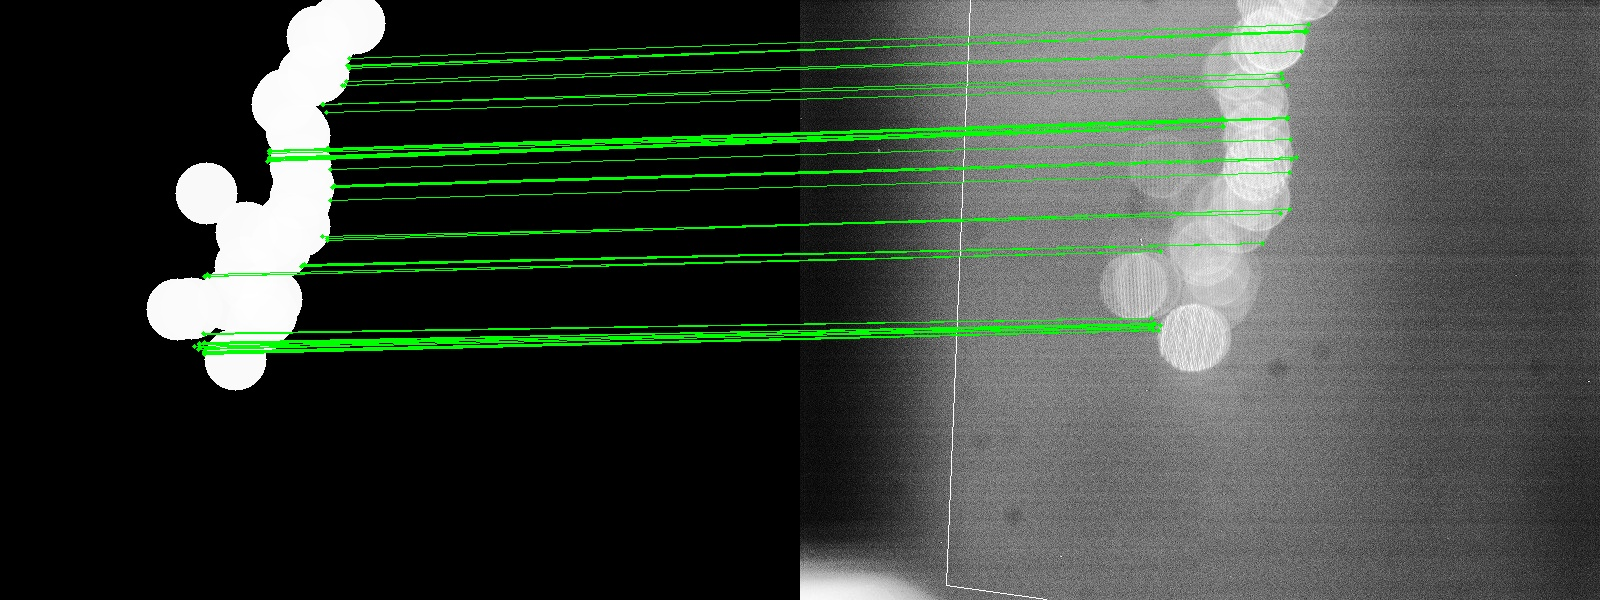
\includegraphics[width=\textwidth]{img/asift-matching.jpg}
    \caption{Matching between focussed and defocussed images.}
    \label{fig:asift-matching}
\end{figure}

\begin{figure}[t]
    \centering
    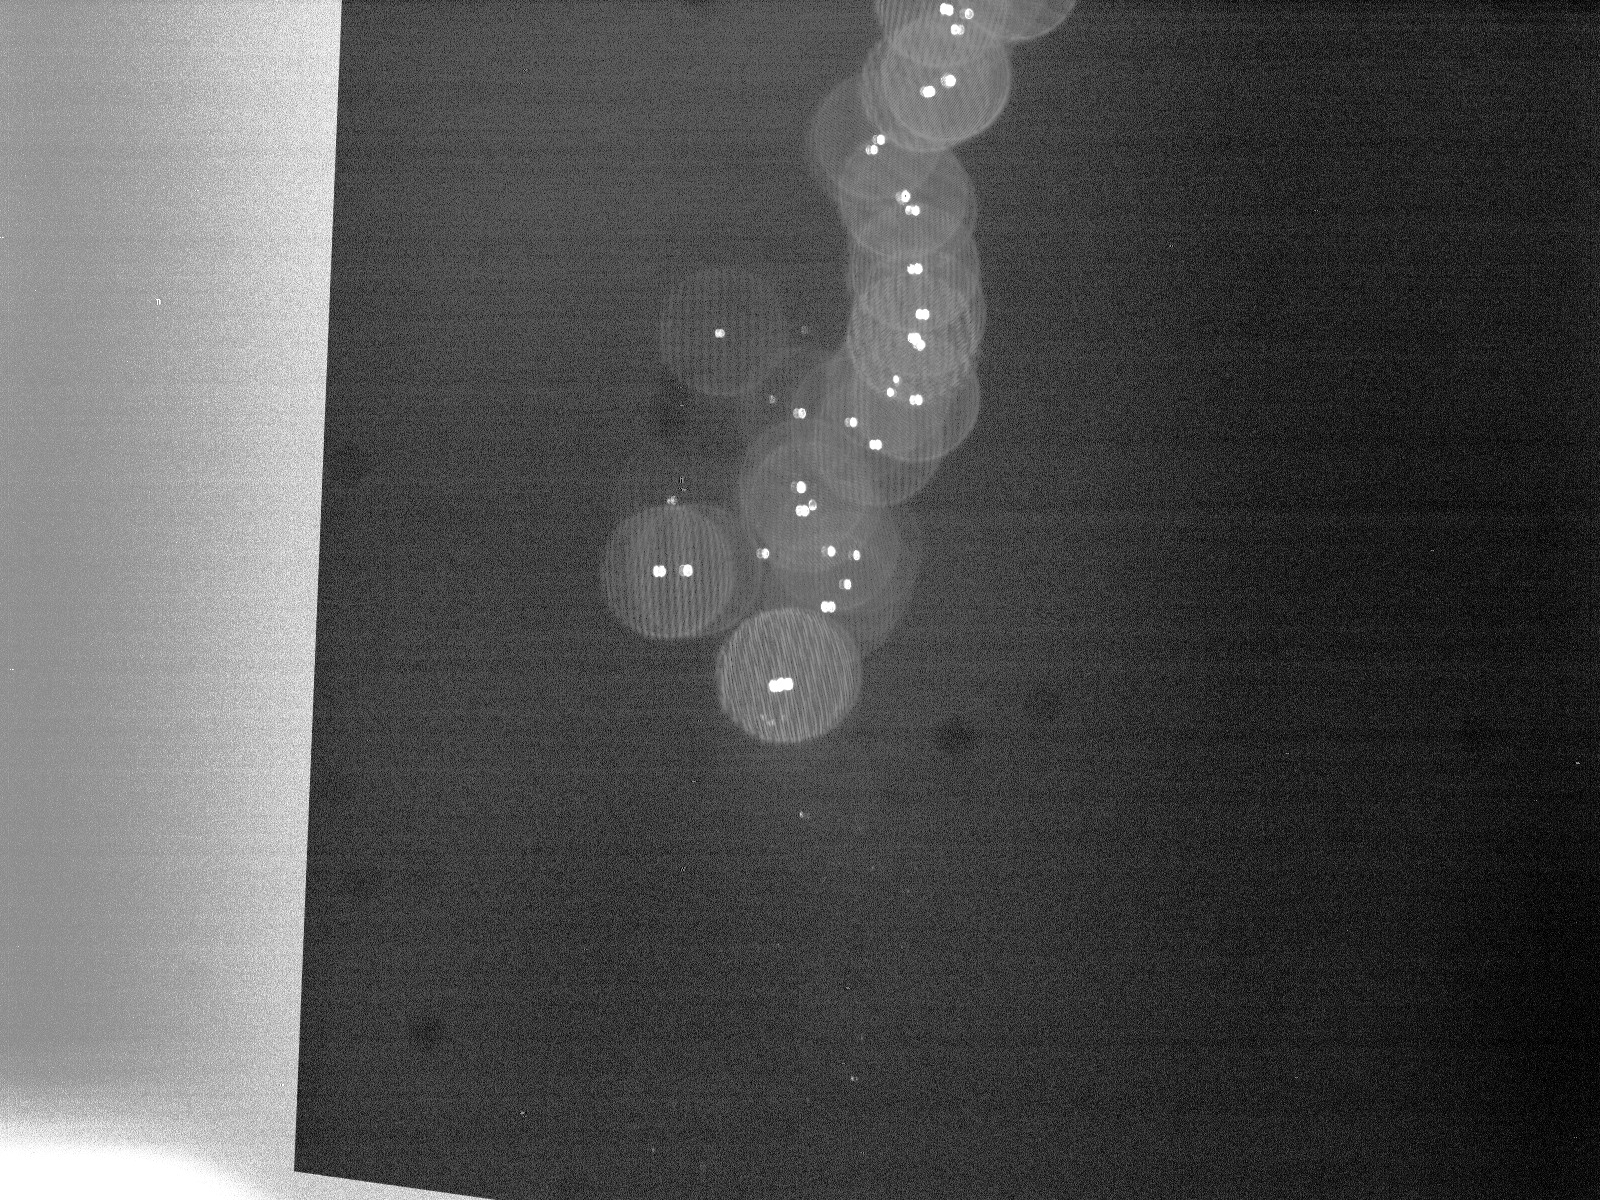
\includegraphics[width=0.45\textheight]{img/drop-calibration-corrected.jpg}
    \caption{Focussed camera image, after applying homography
        derived from image registration, is superimposed onto defocussed
    camera image of droplets.}
    \label{fig:drop-calibration-corrected}
\end{figure}

%%%%%%%%%%%%%%%%%%%%%%%%%%%%%%%%%%%%%%%%%%%%%%%%%%%%%%%%%%%%%%%%%%%%%%%%%%%
%%%%%%%%%%%%%%%%%%%%%%%%%%%%%%%%%%%%%%%%%%%%%%%%%%%%%%%%%%%%%%%%%%%%%%%%%%%
\section{Thin lens assumption}
What matters is the Numerical Aperture (NA), which is (the sine of half of) the
collection angle. When we have a simple lens, we can calculate this as
\begin{equation}
    \mathrm{NA} = \sin \frac{d_a}{2z}\\
    3\alpha \rho = \sqrt{2 \lambda x r}
\end{equation}

The Dantec manual suggests using the distance from light sheet to front of the
lens for $z$, and the ratio of min focal length and max f-number to find $d_a$.
This, however, does not result in an accurate value for the collection angle
with all lenses.

We are assuming, then, that the effective aperture (the entrance pupil) always
stays constant throughout the focussing range of the lens. This is not
necessarily the case, as there are lenses which change both the physical and the
virtual size of the aperture when focussing. The best way to get the collecting
angle is to go by magnification

\subsection{Finding the correct value for aperture diameter}
Here is where I make the claim that it is impossible to determine the actual
exact value for the numerical aperture of the lens. Similarly, it can be quite
difficult to determine the accurate distance from light sheet to lens aperture
(even though the latter measurement is more forgiving, since the distances are
far greater).

\subsection{Error in the Mie approximation at small sizes}
\label{sec:mie-error}
As outlined in paper ... geometric optics deviate from the true Mie scattering
field when sizes are very small.

%%%%%%%%%%%%%%%%%%%%%%%%%%%%%%%%%%%%%%%%%%%%%%%%%%%%%%%%%%%%%%%%%%%%%%%%%%%%%%%
%%%%%%%%%%%%%%%%%%%%%%%%%%%%%%%%%%%%%%%%%%%%%%%%%%%%%%%%%%%%%%%%%%%%%%%%%%%%%%%
%                            SLIT APERTURES                                   %
%%%%%%%%%%%%%%%%%%%%%%%%%%%%%%%%%%%%%%%%%%%%%%%%%%%%%%%%%%%%%%%%%%%%%%%%%%%%%%%
%%%%%%%%%%%%%%%%%%%%%%%%%%%%%%%%%%%%%%%%%%%%%%%%%%%%%%%%%%%%%%%%%%%%%%%%%%%%%%%

\chapter{Particle sizing with \\a slit aperture}
As we discussed in section \ref{sec:ipi-overlap}, many otherwise well-executed IPI
measurements are thwarted by overlapping defocussed droplet images.
This problem is never more apparent than in efforts to calibrate
the system using a vibrating orifice droplet generator, as the droplets produced
thereby are spaced very closely and produce heavily overlapping defocussed
images. Fortunately, there exists a simple and reliable technique to deal with
this problem: a slit aperture, installed directly in front of the lens, masks
the defocussed droplet images such that only a thin strip across their center
passes through the lens. The effect is shown in Figure \ref{fig:globalsizing}. 

The idea of optically compressing an image in one direction is
well-known from the field of spectroscopy. It was first introduced to the area
of fluid measurement by \citet{Durst94}, and has since been employed in various
forms, e.g. by \citet{Pan06}. Other authors use cylindrical lenses instead
of slit apertures to achieve the vertical integration of the image
\cite{Kawaguchi02}.

\begin{figure}[h]
    \centering
    \begin{subfigure}[b]{0.4\textwidth}
        \centering
        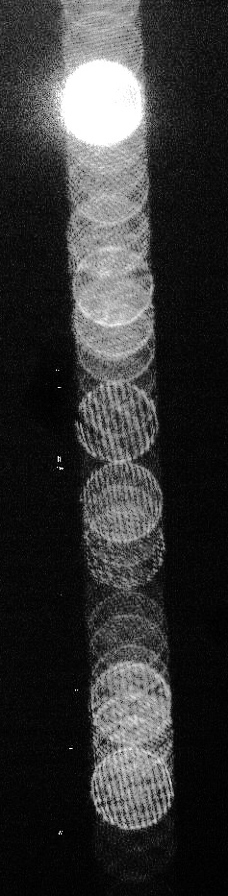
\includegraphics[height=0.6\textheight]{img/dots_cropped.jpg}
        \caption{}
    \end{subfigure}
    \begin{subfigure}[b]{0.4\textwidth}
        \centering
        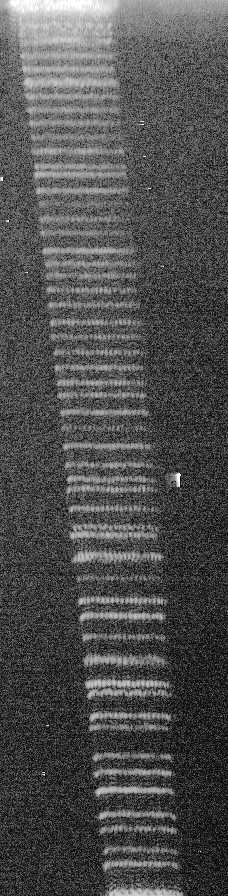
\includegraphics[height=0.6\textheight]{img/slitted.jpg}
        \caption{}
    \end{subfigure}
    \caption{Before (a) and after (b) installing the slit aperture. The aperture
    stop pares off the top and bottom halves of the defocussed circles, leaving
only a narrow center string in the middle.}
    \label{fig:globalsizing}
\end{figure}

\section{Optical theory}
Naturally, equations \eqref{kappa} and \eqref{fringedistance-pixels} still hold.

\section{Image processing}
Extracting the fringe counts from such an image is straightforward. First, we
correlate the image with that of a single, solid bright rectangle which shares
the approximate dimensions of a typical strip in the image. This operation
yields intensity
peaks centered over our regions of interest. We remove closely adjacent peaks,
as they may represent questionable or overlapping strips. Compared to the sheer
number of correctly identified strips, the number of legitimate data points lost
this way is negligible. Figure \ref{fig:globalsizing-identifystrips} shows the
result of such an attempt at identifying the strips.

\begin{figure}[h]
    \centering
    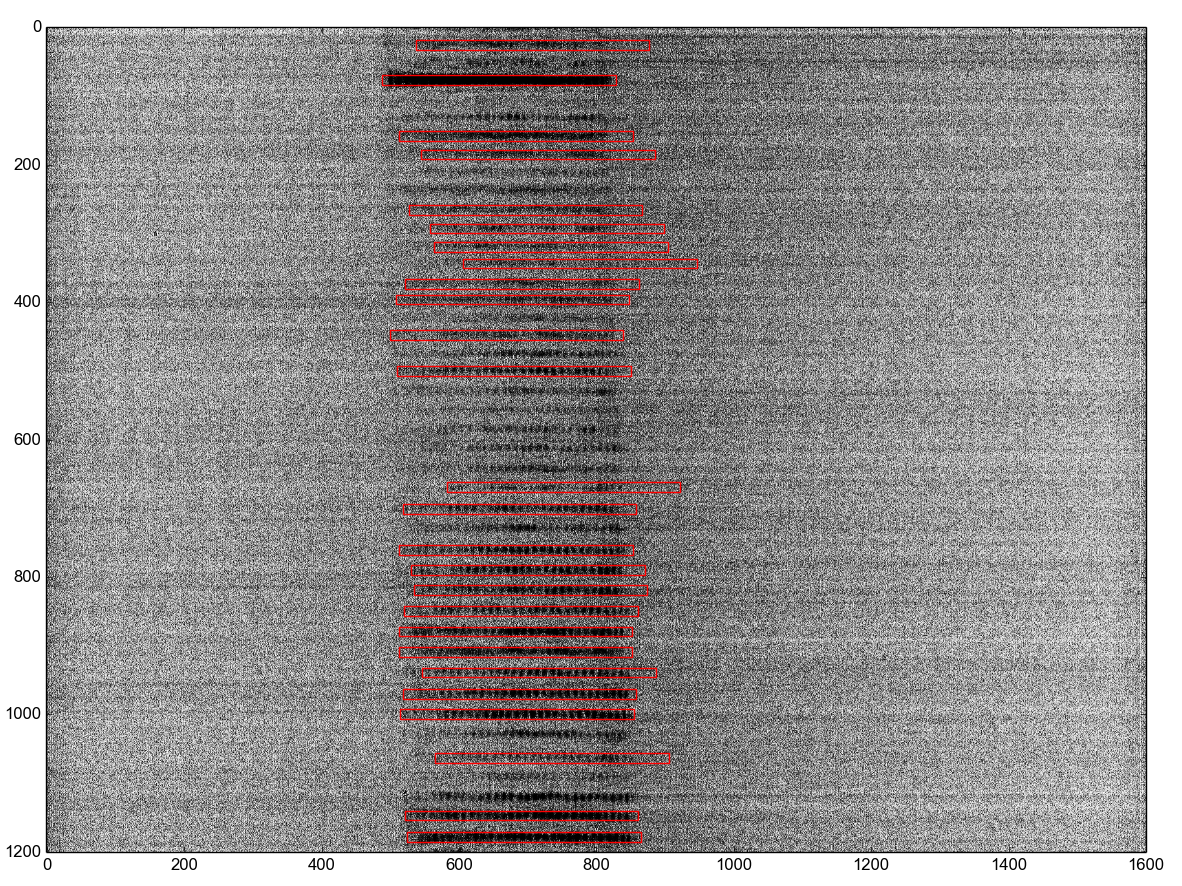
\includegraphics[height=0.38\textheight]{img/globalsizing-identifystrips.png}
    \caption{The image is correlated with that of a solid bright rectangle, which
        results in peaks that approximately coincide with the centres of the
        strips. Here, the original photo is shown with rectangles drawn centered
    at said peaks.}
    \label{fig:globalsizing-identifystrips}
\end{figure}

To find the number of fringes within the strip, we cannot rely on counting the
number of dark/bright variations directly, as some of them may be lost in the
noise. The spatial frequency of the peaks, however, taken together with the
known and constant horizontal width of the strips, will produce a reliable
fringe count. In the next step, our algorithm therefore applies the Fourier
transform to each region of interest. To improve the accuracy of the method,
three steps are performed before the Fourier transform is taken:
\begin{enumerate}
    \item a weak ($3 \times 3$) Gaussian blur is applied to the region
        (optional);
    \item a Hanning window is applied to the region -- both horizontally and
        vertically. This reduces the ``sinc ringing'' effect encountered when
        taking the Fourier transform of finite signals;
    \item the region is padded with zeros in all directions to yield a larger
        input to the Fourier transform. In our application, the windowed and padded strip
        images had dimensions of $1024 \times 1024$ pixels. Zero-padding
        increases the granularity of the frequency spectrum, which can help with
        the correct identification of the peak frequency.
\end{enumerate}

Figure \ref{fig:globalsizing-dropletpeak} shows the windowed appearance of
one such region of interest (although it does not show the padded input to the
Fourier transform due to space constraints). The Fourier transform yields a
frequency power spectrum in two dimensions, although we are primarily interested
in the frequency peak in the horizontal direction (i.e. along $y=0$). In order
to minimize the misidentification of dominant frequencies,
\begin{enumerate}
    \item we clip the spectrum to a band of reasonable frequencies. This is
        necessary because a) $1/f$-noise causes very low frequencies to dominate
        in power, although they are of no interest to us, and b) graininess in
        the original photo can sometimes result in meritless high-frequency
        peaks;
    \item we apply a Gaussian blur to the 2D spectrum to remove outliers in the
        spectrum;
    \item we discard all regions in which the peak frequency's power does not
        exceed a certain value;
    \item we discard all regions in which the \textit{prominence} of the peak
        freqency's power (i.e. its proportion to the mean power) does not exceed
        a certain value (this step is optional).
\end{enumerate}
The bottom two elements in Figure \ref{fig:globalsizing-dropletpeak} illustrate
the effect of these steps.

\begin{figure}[h]
    \centering
    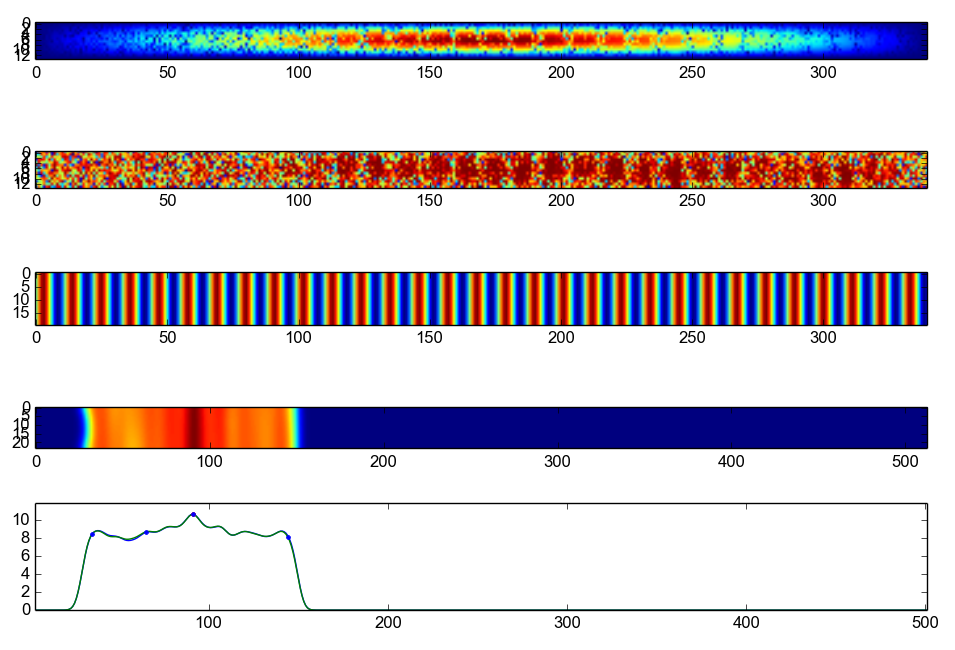
\includegraphics[height=0.38\textheight]{img/globalsizing-dropletpeak.png}
    \caption{From top to bottom: windowed region of interest; original
    (unwindowed) region of interest; sine wave representing the identified peak
frequency; clipped and lowpass-filtered 2D frequency spectrum showing a distinct
peak at about 90 oscillations across the image width of 1024 pixels; 1D plot of
the frequency spectrum, with peak identified at $f=91.0$.}
    \label{fig:globalsizing-dropletpeak}
\end{figure}

Finally, the peak frequency $f_\text{peak}$ is converted into a fringe count by re-scaling it
from the padded size $D_\text{padded}\, (= 1024$ pixels) to the width of the strip (which, in the
context of IPI measurements, should equal the diameter $D_\text{i}$ of the defocussed droplet
image):
\nomenclature{$f_\text{peak}$}{Peak frequency}
\nomenclature{$D_\text{i}$}{Diameter (in pixels) of the defocussed image}
\nomenclature{$D_\text{padded}$}{Width (in pixels) of the padded input to the
Fourier transform}
\begin{equation}
    N_\text{fr} = f_\text{peak} \frac{D_\text{i}}{D_\text{padded}}
    \label{fringes-from-diameter}
\end{equation}

In the current implementation of our algorithm, $D_\text{i}$ must be determined
and entered manually.

\section{Sources of error with the slit method}
\subsection{Misalignment of slit and lens}

While the above algorithm will generally give a good estimate of the fringe
\begin{wrapfigure}{r}{0.35\textwidth}
    \begin{center}
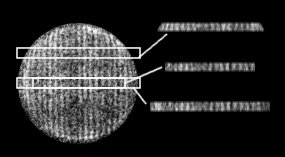
\includegraphics[width=0.33\textwidth]{img/dropletslitcropping2.jpg}
\end{center}
\caption{Only a slit aperture centered on the lens and extending across the
entire lens entrance will preserve all fringes}
\label{fig:droplet-slitcropping}
\end{wrapfigure}

count for a given defocussed droplet image, it cannot know whether the entire
center portion of the image has indeed passed the slit aperture. It is
conceivable, after all, that the slit aperture was not perfectly centered on the
lens entrance, or that the slit aperture was shorter than the diameter of the
lens entrance. Figure \ref{fig:droplet-slitcropping} illustrates how the slit
aperture can cause the defocussed image to appear smaller than it is. The
reduced value for $D_\text{i}$, manually entered in equation
\eqref{fringes-from-diameter}, will result
in droplets being reported as smaller than they are in reality.

\section{Calibrating the slit method}
Taking into account the sources of errors explained in the sections above, it is
advisable to run a few calibration tests with droplets of different sizes before
employing the IPI technique for real spray measurements. Recall that, if we
ignore the Mie error (section \ref{sec:mie-error}), the relationship between fringe count and droplet diameter
is linear with a constant of proportionality $\kappa$ (see equation
\eqref{kappa}). The aim of our calibration, then, is to determine the value of
$\kappa$ from experiment -- the premise being that we cannot be certain of the
values of $D_a$, $z$, and possibly not even $m$ and $\phi$ (although the latter
can usually be ascertained to a sufficient degree of accuracy).

\subsection{A sample calibration of the slit aperture method}
Using the droplet generator described in section \ref{sec:droplet-generator} and
the IPI configuration described in section \ref{sec:ipi-setup}, we produced and
measured monodisperse droplets of many different diameters. The droplet
diameters were determined both mathematically and photographically, as described
in section \ref{sec:verify-droplet-diameters}. Out of over 30 sets of IPI
measurements we selected five sets that exhibited both strong uniformity and
high photographic quality:

\begin{table}[h]
\begin{tabular}{rrrrr}
    \toprule
Flow rate & Freq. & $D_d$, predicted  & $D_d$, from
    photo & $N_\text{fr}$ \\
    \midrule
    20.8  ml/h  & 5395 Hz  & 127 $\mu$m  & 100-126 $\mu$m &  9.6      \\
39.7  ml/h  & 1990 Hz  & 220 $\mu$m  & 203     $\mu$m &  16.5     \\
79.4  ml/h  & 1565 Hz  & 299 $\mu$m  & 290     $\mu$m &             \\
94.3  ml/h  & 1067 Hz  & 361 $\mu$m  &         $\mu$m &  27.2          \\
114.1 ml/h  & 1065 Hz  & 386 $\mu$m  &         $\mu$m &  29.8          \\
    \bottomrule
\end{tabular}
\end{table}

The distributions are shown here:



\subsection{Discussion of Results}
This is where I list my results and discuss what they might mean for
calibration purposes.

\section{Conclusion}
- Conclusion:
    - Dantec's circle detection algorithm is garbage
    - Use a slit aperture instead

\chapter{Phase-Doppler Particle Analysis}
This is on PDPA method.


\bibliographystyle{myplainnat}
\bibliography{bibliography}
\end{document}
